\documentclass{article}
\usepackage{amsmath, amsfonts, amsthm, amssymb}
\usepackage{fullpage}
\usepackage{enumerate}

% For figures
\usepackage{graphicx}
\usepackage{subfigure}

\usepackage{amsmath,amssymb}

\usepackage{hyperref}

%%%%%%%%%%%%%%%%%%%%CONTENT MACROS%%%%%%%%%%%%%%%%%%%%%%%%%
\newcommand{\inv}{^{-1}}                            % inverse operator
\newcommand{\sminus}{\backslash}                    % set minus
\newcommand{\N}{\mathbb{N}}                         % natural numbers
\newcommand{\Z}{\mathbb{Z}}                         % integers
\newcommand{\R}{\mathbb{R}}                         % real numbers
\newcommand{\acro}[1]{\textsc{\MakeLowercase{#1}}}
%%%%%%%%%%%%%%%%%%%%%%%%%%%%%%%%%%%%%%%%%%%%%%%%%%%%%%%%%%%

\usepackage{natbib}
\usepackage[disable]{todonotes}

\begin{document}
\begin{center}
{\bf\Large Extended Abstract: Distributed and computationally efficient belief
propagation based on swarms of foraging bacteria}\\
Shashank Singh, Saket Navlakha, and Ziv Bar-Joseph\\
Machine Learning Department, School of Computer Science,\\
Carnegie Mellon University, Pittsburgh, PA 15213, USA
\end{center}

\section*{Introduction}
There are several cases in which distributed networks need to perform some sort
of joint computation [1]. One such problem is belief propagation, a process in
which distributed agents share their beliefs with other agents so each agent
can determine an appropriate state or action.
Computational solutions for belief propagation involve a set of nodes
performing local computations and sharing their beliefs with neighboring nodes
across weighted edges. Each node is often assigned an initial score or belief
(which can be derived based on local sensing or observation). Starting with
this score nodes propagate information along the edges of the graph until their
(local) belief converges. Belief propagation methods were originally developed
to perform statistical inference in graphical models[2] and are widely used for
image analysis [3], in error correcting codes [4], to assign function to genes
[5], and by sensor networks in remote locations that need to jointly decide
whether a specific event happened (for example,  an earthquake or river
contamination [6]).
 
Standard belief propagation algorithms often require sending large messages
(usually continuous probability values), assume unique identifiability of
senders (since each has a different weight) and require that nodes perform
substantial computations at each iteration [7]. These requirements may be
problematic for distributed sensor or wireless networks that operate under
strict communication and computation constraints and need to conserve energy
and battery life [8], [9]. Coordination and computation over networks is a
shared goal between computational and biological systems [8]. Specifically,
bacterial cells often coordinate using chemotaxis to detect food sources [10].
Given the environments they reside in, these cells need to both move towards
available food sources and avoid obstacles along the way. To achieve this goal
each bacterial cell employs a number of sensors and integrates information from
these sensors to determine its direction and velocity at each time point. These
sensors include gradient detectors that determine food location [11], community
sensors to gather information from other bacteria cells which presumably are
also moving towards the food source and may have already detected (and avoided)
obstacles, and sensors to avoid collisions with nearby bacterial cells.

This process closely resembles belief propagation. On the one hand each cell
has its own belief (the food gradient it detects) but on the other it relies on
information from neighboring cells to refine its trajectory based on possible
obstacles and the beliefs of its neighbors. Recent models for this process [12]
assume both continuous messages (or the equivalent ability to detect detailed
information regarding neighboring cells) and identifiability of these
neighbors, yet both assumptions seem unlikely for real bacteria.

In this work we developed a belief propagation model that solves the bacterial
food search problem while minimizing both communication and computation.
Compared to many prior algorithms for collective navigation based on flocks of
birds [14], and foraging ants [15], our methods do not assume identifiability
of individual agents and uses sparse communication while still being able to
handle complicated environments with several other cells and obstacles. The
limited computation and communication model we assume makes this method
appropriate to other problems in which severe constraints exist on these
resources. 

\section*{Methods}
We first briefly describe the model introduced by Shklarsh et al. [12], which
attempts to explain how swarms of bacterial cells coordinate food search. Next,
we describe our low complexity communication algorithm based on the stone-age
distributed communication model [16].

\subsection*{The Shklarsh et al. Model}
The model assumes that four issues affect the movement of an individual cell:
(1) The cell’s own sensing of the food gradient; (2) Repulsion from very close
cells to avoid collisions; (3) Velocity adjustments based on cells that are
close, but not too close; and (4) Alignment (in terms of trajectory) with cells
that are further away to avoid group fragmentation. Except for (2) above, which
deals with physical constraints in terms of possible movement, the other issues
all attempt to combine local (personal) and global (population wide)
information to determine the best speed and direction for the next step. Note
that by relying on cells that are (presumably) further along in their food
search allows an individual cell to avoid potential obstacles that it cannot
observe on its own.

The model assumes that cells can determine specific speeds and location for all
other cells (an assumption we will relax in the next section). Given these
observations, at each time step, each cell's movement is computed as an equally
weighted sum of three factors: (1) the cell's previous velocity weighted by the
current food gradient (i.e., the change in food density at the current time
step from the previous time step); (2) displacement and velocity information
communicated by neighboring cells and (3) internal movement noise, modeled as a
zero-mean Gaussian perturbation of the movement direction. Factors 1 and 3 are
internal to the cell while factor 2 is based on communication with other cells
and is computed in the following way: when an agent has a neighbor within the
radius of repulsion, the communication term $u_i$ is set to
\begin{equation}
u_i = - \sum_{x_j \in B_{RR}(x_i)} \frac{x_j - x_i}{\|x_j - x_i\|}.
\label{eq:repulsion}
\end{equation}
Otherwise, the communication term is
\begin{equation}
u_i = \sum_{x_j \in B_{RO}(x_i)} v_j
    + \sum_{x_j \in B_{RA}(x_i)\sminus B_{RO}(x_i)}
                                \frac{x_j - x_i}{\|x_j - x_i\|},
\label{eq:orient_plus_attract}
\end{equation}
where $x_i \in \R^2$ and $v_i \in \R^2$ are the position and velocity of agent
$i$, $B_R(x_i)$ denotes the ball of radius $R$ centered at $x_i$ (Figure
\ref{fig:comm}), and $\|\cdot\|$ denotes Euclidean distance. Following this
calculation, collision avoidance is first used to adjust the movement in the
opposite direction using Equation (\ref{eq:repulsion}) above. If there are no
other cells within distance $RR$, the cell moves according to a weighted sum in
Equation (\ref{eq:orient_plus_attract}) above.
%%%BEGIN FIGURE%%%
\begin{figure}[h!]
\begin{center}
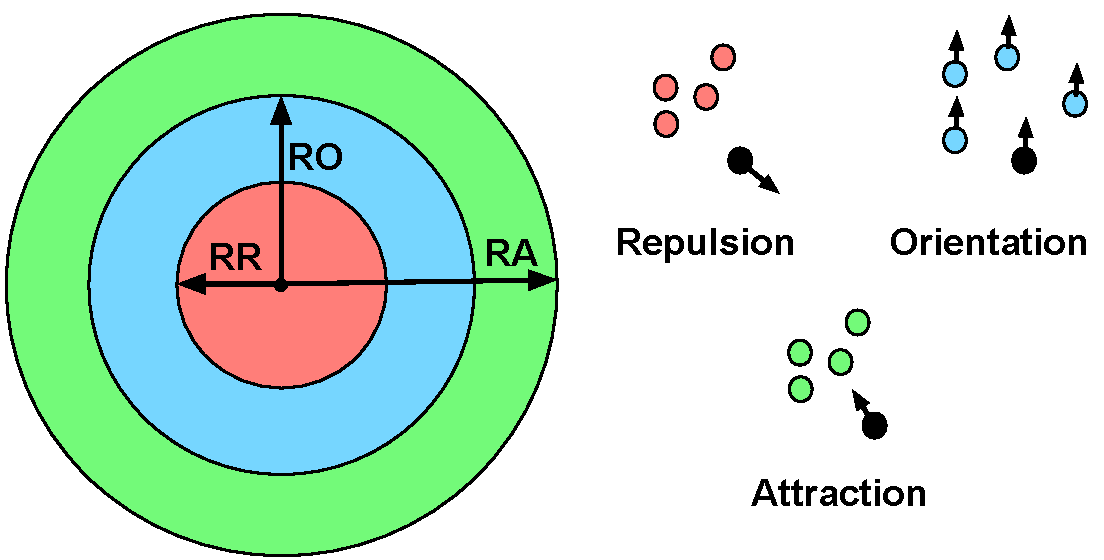
\includegraphics[width=0.5\textwidth,natwidth=610,natheight=642]{comm.pdf}
\end{center}
\vspace{-3mm}
\caption{Dynamics of repulsion, orientation, and attraction for a single
bacterial cell.}
\label{fig:comm}
\end{figure}
%%%%%END FIGURE%%%

\subsection*{A more realistic and computationally efficient model}
A major computational difficulty in the Shklarsh model is that interactions are
highly dependent on communication of exact displacement and velocity between
cells. Each agent A must know the radius (RR, RO, and RA) in which each other
agent B lies, and, based on this, move in a direction away from, parallel to,
or toward B. Furthermore, this information is assumed to be communicated with
fidelity independent of the actual distance between agents (Equations
(\ref{eq:repulsion}) and (\ref{eq:orient_plus_attract}) above both sum unit
vectors). For real cells, this information is communicated via secretion and
detection of chemicals which diffuse indistinguishably (i.e., chemicals
secreted by one cell are indistinguishable from those secreted by another).
Hence the information available to a cell is actually a gradient of attractive
and repulsive chemicals. Also, while a cell may be able to distinguish between
some concentration levels, it is unlikely that it can use continuous values,
and it certainly cannot determine the number of other cells present, which is
required, for example, on the right hand part of Equation
(\ref{eq:orient_plus_attract}). We propose a new model that improves upon the
Shklarsh model in the following ways:
\begin{enumerate}[a)]
\item {\bf Discrete vs. continuous values:} We use a reduced set of discrete
messages, and do not assume that cells know the number of active cells in the
swarm.
\item {\bf Anonymity:} We do not assume that cells can uniquely identify the
sender of any message.
\item {\bf One-two-many communication:} We use a formal communication model
used to analyze biological systems: stone-age distributed computing [16]. This
model allows each cell to only count up to a small threshold value.
\item {\bf Distance-based weighting:} We assume the influence of a neighbor on
the orientation and attraction components of interaction decays with distance.
\end{enumerate}
In our model, if an agent has a neighbor within the radius of repulsion, the
communication term in Equation (\ref{eq:repulsion}) simply sums up the number
of cells within this radius without relying on their exact location. For
Equation (\ref{eq:orient_plus_attract}) we use the following modification:
\begin{equation}
u_i = \sum_{x_j \in B_{RO}(x_i)} \frac{D_{L,T}(\|v_j\|)}{\|x_j - x_i\|}
                                \cdot r\left( v_j \right)
    + \sum_{x_j \in B_{RA}(x_i)} \frac{D_{L,T}(\|x_j - x_i\|)}{\|x_j - x_i\|}
                                \cdot r\left( x_j - x_i \right),
\label{eq:our_orient_plus_attract}
\end{equation}
where $L$ is a positive integer denoting the number of communicable velocity
levels, $T$ denotes the stone-age computing threshold, $D_{L,T}$ denotes the
discretization and thresholding (using the stone age model) function, and
$r : \R^2 \to \R^2$ denotes a vector ``rounding'' function that best
approximates an input vector by one of eight unit-length cardinal vectors
($[\pm1,0],[\pm\sqrt2,\pm\sqrt2],[0,\pm1]$).

Under this model, bacteria need only $3 + \log_2 L$ bits to communicate
velocity or attraction information ($\log_2 8$ bits for direction and
$\log_2 L$ bits for magnitude). The contribution of neighbors at distance $d$
also decays as $d\inv$, so that further away cells have reduced impact. On the
other hand, cells no longer need to know the precise radius ($RO$ or $RA$)
within which each neighbor falls, since we remove the set difference from the
second sum in Equation (\ref{eq:orient_plus_attract}).

\section*{Experiment}
We compared the original Shklarsh et al. model
to these 3 modifications. The first modification ('weighted') incorporated the 
weighting components for orientation and attraction. The second modification
('discrete') incorporated the $L$ level discretization and $T$ threshold
components of Equation (\ref{eq:our_orient_plus_attract}) for orientation. The
third modification is just the combination of the previous two (discretizing
before weighting). 

{\bf Setup:}
We used a swarm of $n = 50$ cells, radii $RR = 0.1$, $RO = 2$, and $RA = 5$,
noise with $\sigma = 0.5$. For discretized models, we used $L = 4$ and $T = 1$,
reducing orientation information communicated to 5 bits.

{\bf Testbed:} Food density and terrain were treated as constant over
time. Food density was modeled as a $0$-order modified Bessel function of the
second kind $K_0$ (the solution to a system of differential equations modeling
diffusion from a point source). The swarm is searching for the global maximum
(the food source) of the density. In addition, we introduce obstacles in the
form of local minima. In particular, we use the following field of
obstacles:
\begin{equation}
f(x) = c_1K_0(\|x\|) + \min(0,\cos(x_1)\cos(x_2) + c_2).
\label{eq:terrain}
\end{equation}
where $c_1$ and $c_2$ are small positive constants. Some additional obstacles
in the forms of parabolic local minima were also added manually. The swarm was
initialized by placing cells uniformly at random in a predetermined region. In
experiments involving a second swarm, the second swarm was placed in the same
manner once the first swarm had located the food source.

{\bf Evaluation:} We measure performance of the algorithm on a
particular trial by the mean path length; i.e., the number of iterations before
the mean of the swarm is within a small radius of the food source. 

\section*{Results}

For each of 300 trials of each model, we recorded (a) the number of iterations
required to find the food source (path length) and (b) the distance from the
food source at each iteration (see Figure \ref{fig:res}). The weighted
versions of the model perform significantly better, each converging 1.5-2 times
faster than the corresponding unweighted version. In particular, the weighted
versions are much better at maneuvering around obstacles, for which bacteria
are best informed only by their immediate neighbors rather than further
neighbors who have, for instance, already traversed the obstacle. Surprisingly,
the simplified (discrete) communication models also perform better than the
corresponding continuous version. This may be because communicated velocity is
denoised by rounding down, since only agents relatively confident in their
direction are fast moving.


%%%BEGIN FIGURE%%%
\begin{figure}[h!]
\begin{tabular}[h]{cc}
\centering
\includegraphics[width=0.5\textwidth]{length_distributions.png}
    & \includegraphics[width=0.5\textwidth]{distance_over_time.png}\\
Path Length (iterations)
    & Iteration
\end{tabular}
\vspace{-3mm}
\caption{(a) Distribution of mean path lengths and (b) average distance from
food source over time, for each model.}
\label{fig:res}
\end{figure}
%%%%%END FIGURE%%%

We also studied the effect of a bacteria swarm already at the food source on a
second swarm of the same size as it searches for the food source from the
same starting location. Results are qualitatively similar to the results
presented in Figure 2, with the weighted discrete version outperforming all
other versions. However, the second swarm consistently converges to the food
source more quickly, since it can rely on information from the first swarm.
Detailed results for the second swarm are omitted for lack of space. 

To conclude, our low complexity communication model improves over current, more
complex computational methods and may enable more efficient belief propagation
in distributed and noisy environments.

\section*{References}
[1] J.-Y. Chen, G. Pandurangan, and D. Xu, ``Robust computation of aggregates in
wireless sensor networks: distributed randomized algorithms and analysis,'' in
Proceedings of the 4th international symposium on Information processing in
sensor networks, Piscataway, NJ, USA, 2005.\\[8pt]
[2] T. Hastie, R. Tibshirani, and J. Friedman, The Elements of Statistical
Learning. New York, NY: Springer New York, 2009.\\[8pt]
[3] P. F. Felzenszwalb and D. P. Huttenlocher, ``Efficient belief propagation
for early vision,'' in Proceedings of the 2004 IEEE Computer Society Conference
on Computer Vision and Pattern Recognition, 2004. CVPR 2004, 2004, vol. 1, pp.
I–261–I–268 Vol.1.\\[8pt]
[4] E. R. Ackermann, T. L. Grobler, A. J. Van Zyl, and J. C. Olivier, ``Belief
propagation for nonlinear block codes,'' in AFRICON, 2011, 2011, pp. 1–6.\\[8pt]
[5] S. Letovsky and S. Kasif, ``Predicting protein function from protein/protein
interaction data: a probabilistic approach,'' Bioinforma. Oxf. Engl., vol. 19
Suppl 1, pp. i197–204, 2003.\\[8pt]
[6] Keat G. Ong, Xiping Yang, Niloy Mukherjee, Haidong Wang, Shrawan Surender,
and Craig A. Grimes, ``A Wireless Sensor Network for Long-term Monitoring of
Aquatic Environments: Design and Implementation,'' Sens. Lett., vol. 2, no. 1,
pp. 48–57, 2004.\\[8pt]
[7] M. Mzard and A. Montanari, Information, Physics, and Computation. Oxford ;
New York: OUP Oxford, 2009.\\[8pt]
[8] S. Navlakha and Z. Bar-Joseph, ``Algorithms in nature: the convergence of
systems biology and computational thinking,'' Mol. Syst. Biol., vol. 7, p. 546,
2011.\\[8pt]
[9] J. Carle and D. Simplot-Ryl, ``Energy-efficient area monitoring for sensor
networks,'' Computer, vol. 37, no. 2, pp. 40–46, Feb. 2004.\\[8pt]
[10]    D. Claessen, D. E. Rozen, O. P. Kuipers, L. Søgaard-Andersen, and G. P.
van Wezel, ``Bacterial solutions to multicellularity: a tale of biofilms,
filaments and fruiting bodies,'' Nat. Rev. Microbiol., vol. 12, no. 2, pp.
115–124, Feb. 2014.\\[8pt]
[11]    R. M. Macnab and D. E. Koshland Jr, ``The gradient-sensing mechanism in
bacterial chemotaxis,'' Proc. Natl. Acad. Sci. U. S. A., vol. 69, no. 9, pp.
2509–2512, Sep. 1972.\\[8pt]
[12]    A. Shklarsh, G. Ariel, E. Schneidman, and E. Ben-Jacob, ``Smart Swarms
of Bacteria-Inspired Agents with Performance Adaptable Interactions,'' PLoS
Comput Biol, vol. 7, no. 9, p. e1002177, Sep. 2011.\\[8pt]
[13]    I. D. Couzin, J. Krause, N. R. Franks, and S. A. Levin, ``Effective
leadership and decision-making in animal groups on the move,'' Nature, vol. 433,
no. 7025, pp. 513–516, Feb. 2005.\\[8pt]
[14]    B. Chazelle, ``Natural algorithms and influence systems,'' Commun. ACM,
vol. 55, no. 12, p. 101, Dec. 2012.\\[8pt]
[15]    M. Dorigo and C. Blum, ``Ant colony optimization theory: A survey,''
Theor. Comput. Sci., vol. 344, no. 2–3, pp. 243–278, Nov. 2005.\\[8pt]
[16]    Y. Emek and R. Wattenhofer, ``Stone age distributed computing,''
Proceedings of the 2013 ACM symposium on Principles of distributed computing
Pages 137-146, 2013.
\end{document}
